% Written by src/detection/final_figures.py; needs \usepackage{graphicx} and results/figures/ in \graphicspath.
\begin{figure*}[tb]
  \centering
  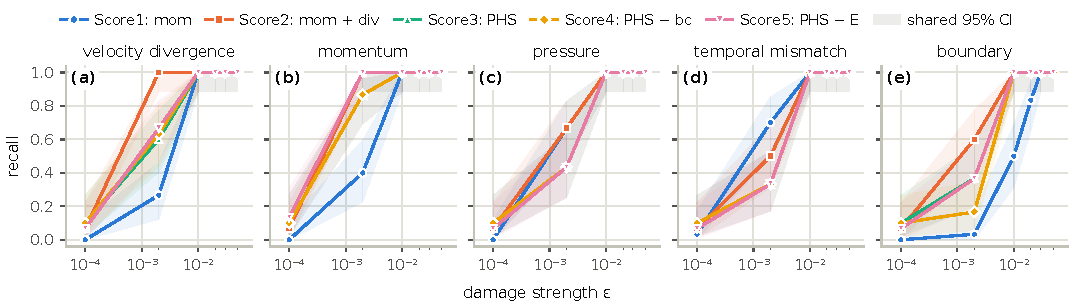
\includegraphics[width=\textwidth]{fig_recall_vs_eps.pdf}
  \caption{Recall of the damaged fields of the 30 new cases against the damage strength $\varepsilon$ (0.0001, 0.002, 0.01, 0.02, 0.03, 0.05; log scale), one panel per damage type and one line per score. A field is flagged when its score is above the frozen $\tau$. Each point is out of 30 fields, one per case; bands: exact (Clopper--Pearson) 95\% confidence intervals, drawn once in grey where several scores have the same count and so the same interval. Every score flags every damaged field from $\varepsilon = 0.01$ on (already from 0.002 for Score2 with velocity divergence and momentum damage and Score5 with momentum damage), except Score1 for boundary damage (15/30 at 0.01 and 25/30 at 0.02). At $\varepsilon = 0.0001$ nearly all flagged fields belong to cases whose clean field the score already flags (10 of 10 for Score2, 15 of 15 for Score3, 15 of 15 for Score4 and 10 of 12 for Score5; Score1, which flags no clean field, flags 1 field there); Fig.~\ref{fig:recall_vs_eps_new_detections} leaves those cases out. Score terms: mom, the momentum residual; div, the continuity residual; bc, the boundary-localization term; E, the energy-decay term; PHS, the sum of all four, each divided by its mean over the calibration fields.}
  \label{fig:recall_vs_eps}
\end{figure*}
